\chapter{Function evaluation}

The key purpose of the Scala Adaptive framework is to always invoke a function that is expected to have the best performance possible in given environment and with given inputs. By \textit{function performance} we mean any measurable description of the qualities of the function. It can be the actual runtime of the function, memory consumption, number of I/O operations, number of threads created, etc. All these factors can be valued and be the goal of the system run optimization.

This thesis is focused on the task of optimizing the function runtime or time complexity in general. The core of the framework, however, is designed to be extensible by modules that can analyze the function run in different ways. More on this topic will be covered in %TODO: REFERENCE

\section{Selection and invocation process}

Suppose we have a combined function \inlinecode{f()} created using the API described in chapter \ref{chapter:api} by combining multiple functions \inlinecode{f1()}, ..., \inlinecode{fn()}. We have a new function (or a function-like object) that can be invoked\footnote{In Scala terms applied} and we expect it to run one of the functions \inlinecode{f1()}, ..., \inlinecode{fn()}.

The basic steps required to do so are the following:

\begin{enumerate}
	\item Locate the runtime history data of \inlinecode{f1()}, ..., \inlinecode{fn()}
	\item Select the function \inlinecode{fk()} to be invoked
	\item Invoke \inlinecode{fk()} and evaluate its runtime
	\item Update the runtime history data of \inlinecode{fk()} with the new record
\end{enumerate}

\subsection{Runtime evaluation}

When talking about function runtime (or an execution time of a function), there are two types of values that we could be evaluating:

\begin{itemize}
	\item \textbf{\textit{Wall clock time}} - time elapsed between entering and leaving the function
	\item \textbf{\textit{CPU time}} - time that the CPU actually spent executing our function
\end{itemize}

The \textit{wall clock time} is always higher than the \textit{CPU time}, because it includes not only the time when CPU is executing the function code, but also the time when the executing thread is waiting for its turn in time-sharing multitasking OS or sleeping on a blocking I/O\footnote{Input / Output operation} operation, synchronization primitive, or for some other reason. This means that the \textit{wall clock time} also gets affected by concurrently running processes, network load, and other environment-based factors, and tends to vary much more between multiple invocations.

For the purposes of the ScalaAdaptive framework, it might seem that the \textit{CPU time} would be more appropriate, as it gives clearer results not affected by the state of the executing environment. The truth is, however, that many of the use cases of the framework require the thread sleeping time to be included in the measurement, as the functions runtimes are determined mainly by the duration of an I/O operation (e.g. database queries, network requests, etc.), so using \textit{CPU time} wouldn't give us the necessary results.

It is also quite difficult to determine the \textit{CPU time} - it requires support from the executing system with tracking the time that every thread has spent in execution. For this reason and for the reason stated above, the selection process in this text is based on \textit{wall clock time}. It might be, however, interesting as a future extension to implement measuring both of the times and allowing the user to select for each combined function which time should be measured.

The \textit{wall clock time} is measured by fetching high-precision system time in nanoseconds right before calling the function apply method and right after returning from the call. The result is the runtime in nanoseconds. This measurement is precise enough for all the use cases of the framework, because it's targeting functions with non-negligible time complexities.

\subsection{Storing the evaluation data}

After having invoked the function and evaluated its runtime, the evaluation data have to be stored before passing the return value back to the caller. Multiple types of storage can be used for that.


\section{Selection strategies}

The most complicated task of the entire chain is to select the most appropriate function to run in given case. The case is described by an input \inlinecode{in} of the function \inlinecode{f()} and by the evaluation data gathered in previous runs.

The most straightforward approach would be to look at the function run history and select the function with the lowest average runtime in the measured runs. This solution has a few problems. First of all, the runtime of the inner functions \inlinecode{f1()}, ..., \inlinecode{fn()} might depend on the input \inlinecode{in}, which could lead to incorrect assumptions if the historical data were measured on runs with various inputs. And secondly, the method doesn't solve the case where the data don't give us an exact answer, for example if there are too few, if the historical results are too scattered (which might have been caused by different conditions upon invocation, etc.), and in general when we can't make a clear decision and need to collect more data instead.

The \textit{input dependency} problem might be solved in various ways. Methods to analyze the relation between the input and the runtime might be employed in order to predict an approximate runtime on a new input. We call these methods \textit{predictive strategies}. A simpler approach that can be used universally with any \textit{non-predictive strategy} without changing it dramatically is to apply it on a smaller subset of the history records that have inputs of a very similar size. 

As for the \textit{uncertainty} problem, the key is to collect a fixed amount of data first before using any of the strategies. Additionally, a techniques from statistical testing can be used so that the strategy could have a maximal probability of an error (a wrong decision).

Based on these observations, a couple of strategies to select function were proposed and implemented as a part of the ScalaAdaptive framework. The user of the framework can decide by himself on which one to use.

\subsection{Predictive strategies}

These strategies are useful solely for the purpose of the functions for which the runtime is directly related to the input of the function, e.g. size of a data structure, length of a data file, a number, etc. The computational complexity of algorithms is usually expressed as a function of the size of the algorithm's input. The actual runtime depends on the complexity, as every computational step has to take some CPU time. 

The problem is that in reality, the duration of different steps differ as well, depend on hardware optimization, cache misses, pagefaults, scheduling of the OS and many other factors, so the relation, although still present, gets very distorted. For the purposes of only approximate predictions in order to determine faster function, we will suppose that for function \inlinecode{f()} \(\exists g\) so that 
\(\forall in\) possible inputs holds \(t = g(in)\), where \(t\) is the runtime on input \(in\) of \inlinecode{f()}.

The input, as mentioned earlier, can be a complex structure with a lot of factors contributing to the runtime\footnote{Consider for example a general graph - for most of the algorithms, both number of vertices and edges have to be taken into account}. For the simplicity of the strategies, we need to introduce an \textit{input descriptor} - an integer that can be computed from the input and that can be used as an input for the function approximation. In other words, we suppose that for function \inlinecode{f()} \(\exists h, g_1\) so that
\(g = h \circ g_1\) 
and 
\(\forall in \quad h(in) \in \mathbb{N}\). In this case, the \textit{input descriptor} of input \(in\) would be the value of \(h(in)\).
This assumption is not true in general, but in most cases, a sufficient function \(h\) can be found so that the results will be precise enough. We call it the \textit{descriptor function}

The \textit{descriptor function} has to be provided by the user of the framework. %TODO: reference to API?
Such function could be:
\begin{itemize}
	\item Number of elements in a data structure argument
	\item Sum of numbers of vertices and edges in a graph
	\item Size of a data file
	\item Identity, if the input is an integer determining the complexity (such as factorial, Fibonacci sequence, etc.)
\end{itemize}
Naturally, the \textit{descriptor function} itself shouldn't have a significant complexity, as it is going to be invoked during every call.

The task of the strategies listed in this section is to make an approximation of the \(g_1\) function and use it to compute \(g_1(h(in))\) upon every invocation and to select the function with the best (minimal) result.

\subsubsection{Simple linear regression}

First strategy supposes that the function \(h\) can be approximated precisely enough using a linear function \(h'\) in the following form:
\[h'(x) = \alpha' x + \beta'\].

This approximation is a \textit{simple linear regression model}. The slope \(\alpha'\) and intercept \(\beta'\) of the linear function can be determined using a least squares method, which minimizes the squares of the distances of the actual function values from the ones predicted by the model.

A big advantage of the model is its simplicity and thus minimal overhead when generating the regression during the selection process. 

The main problem is that the linear regression model applied to a case where the relation is not linear leads to a non-trivial errors that increase with the range that we're trying to cover with the model. Figure \ref{fig:selection_sort_linear_trendline} shows samples of run times of the basic selection sort algorithm, which has the complexity of \(O(N^2)\), on sample arrays with 0 to 30000 integers. Collected data obviously match the quadratic function graph marked with the green color. The red line shows the linear regression model. As we can see, the predictions based on this model would be quite inaccurate, especially if we tried to predict run time on an input significantly larger than the samples.

\begin{figure}[h!]
	\centerline{\mbox{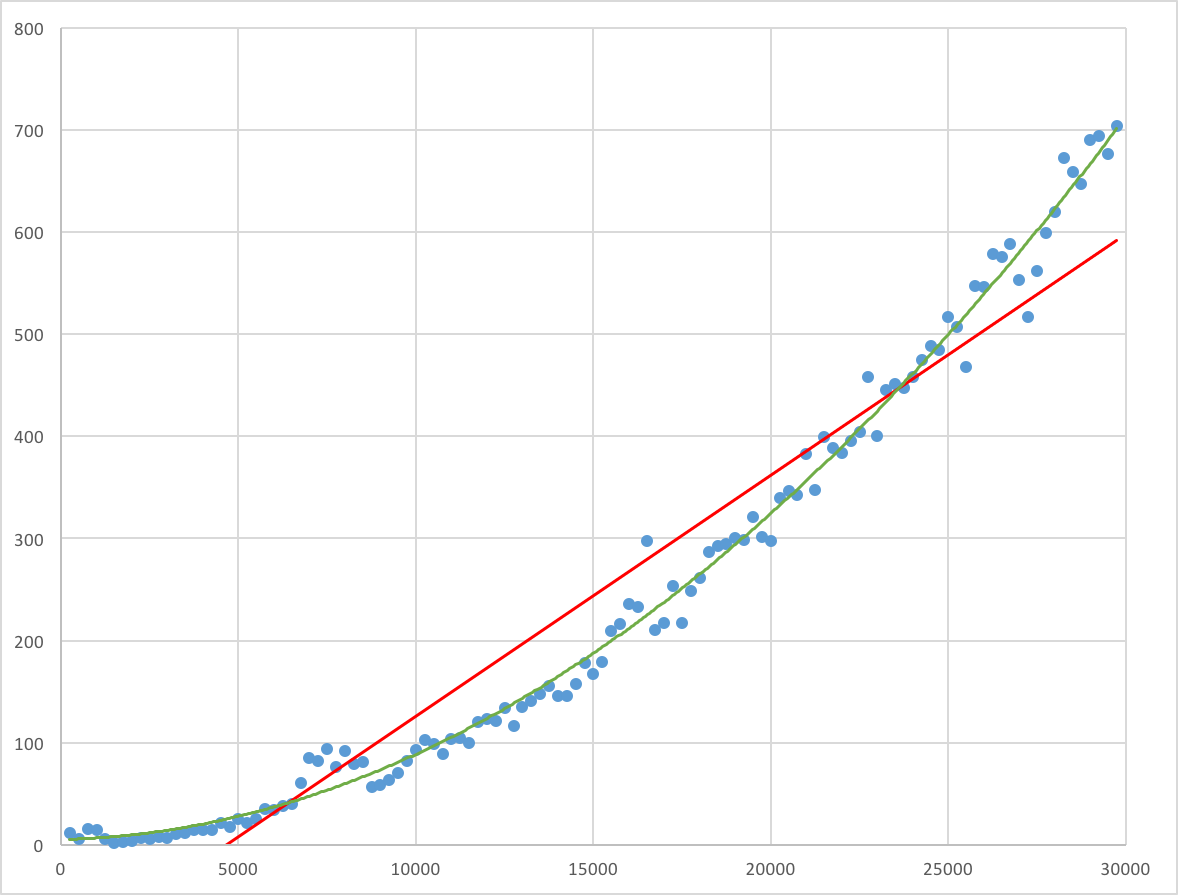
\includegraphics[width=90mm]{./img/selection_sort_linear_trendline.png}}}
	\caption{Linear regression line (red) of a selection sort runtime samples.}
	\label{fig:selection_sort_linear_trendline}
\end{figure}

In order to know the accuracy of the model, we can perform statistical tests on it. We can test the true slope \(\alpha)\) of the hypothetical original linear function, against a constant value \(\alpha_0\). Suppose we have a linear regression model \(h'(x) = \alpha' x + \beta'\) constructed using \(n\) data samples \(x_i, y_i\) (in our case, \(x_i\) are the input descriptors and \(y_i\) are the run times). The hypotheses would be the following:

\[H_0: \alpha = \alpha_0 \]

\[H_1: \alpha \neq \alpha_0 \]

The test statistics \(T\) for the test can be computed using the following formula:

\[T = \frac{\alpha' - \alpha_0}{se(\alpha')}\]

where

\[se(\alpha') = \sqrt{\frac{\sqrt{MSE}}{ \sqrt{ \sum_{i = 1}^{n} (x_i - \bar{x})^2 }}} \]

and

\[MSE = { \sum_{i = 1}^{n} (y_i - y_i')^2 }\]

The \(\bar{x}\) is the average of \(x_i\) and \(y_i' = h'(x_i)\).

Now, the \(T\) follows a \textit{t-distribution} with \(n-2\) degrees of freedom, so \(H_0\) is not rejected on the significance level

\subsubsection{Window-bound linear regression}

\subsubsection{Function interpolation}

\subsubsection{Model construction}

The methods that were described so far are examples of the blackbox techniques - they don't analyze the function itself, they base all their predictions only on the runtime.

More thorough predictions could be made after reaching the function code as well. It can be analyzed, key structures in the code identified (loops, branches, function calls, variables) and a model can be created using these information. The code can be instrumented and the measurement can be done for each of the structures mentioned. 

The prediction will then be based on the model and the data measured for its elements.

This approach has a few problems concerning our intended use cases. The model won't add any value to the predictions if the majority of the execution time will be spent waiting on an I/O operation. Specifically, it won't help with any of the cases where we are selecting a database query, remote server to connect to, etc.

This approach wasn't implemented in our library, because it would require more architectural changes and an appropriate framework for analyzing and instrumenting the code. It could be based on [Predicting Execution Time of Computer Programs].

\section{Selection strategies within a bucket}

\subsection{Statistical tests}

If we assume that the measured function run times come from a normal distribution, we can use methods of statistical testing to determine whether one function is faster than the other with given certainty. 

\subsubsection{Deciding between two functions}

Let's suppose we have two data samples 

\subsubsection{Deciding between multiple functions}


The fact that the actual distribution of the function run times most likely won't be normal can be 

\section{Cross-bucket selection}

\section{Function runtime prediction}

\subsection{Function interpolation}

\section{Experimental behavior with performance limits}
Using available time to "obtain" more data

%TODO - when do I need more data?